\chapter{Appendix for Chapter 4}\label{AppE}
\myappendices{Appendix \ref{AppE} }%\byname{AppA}}
\section{Transposase enrichment in incomplete prophages.}
As described in the main text, we simulated the prophage population with parameter values $r_S = 1.5, \, r_D =0.048 , \, r_L =1.5,  \, r_T = 0.002$ for 5000 generations to compare the gene content of intact and incomplete prophages.  Using a strict definition for ``intact" prophages, that is, only prophages containing all the genes required for excision and re-infection were considered intact, transposase genes were enriched nearly 400-fold in incomplete prophages (see Figure~\ref{fig:Biresultso}) (A) and (B). When the classification of ``intact'' prophages was relaxed to prophages that contain 90\% or more of the possible prophage genes, the results showed a 5.6-fold increase in transposase genes (see Figure~\ref{fig:Biresultso}) (C) and (D). 
\begin{figure}[H]
    \centering
     \begin{subfigure}[t]{0.50\textwidth} 
    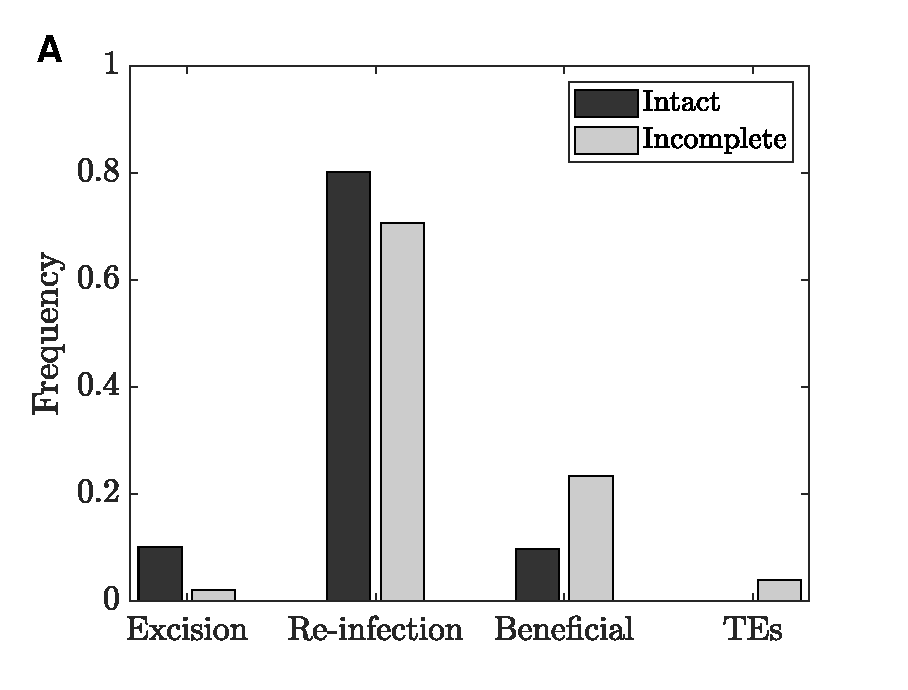
\includegraphics[scale=0.50]{BiTe1o}
     \end{subfigure}\hfill
         \begin{subfigure}[t]{0.50\textwidth}
    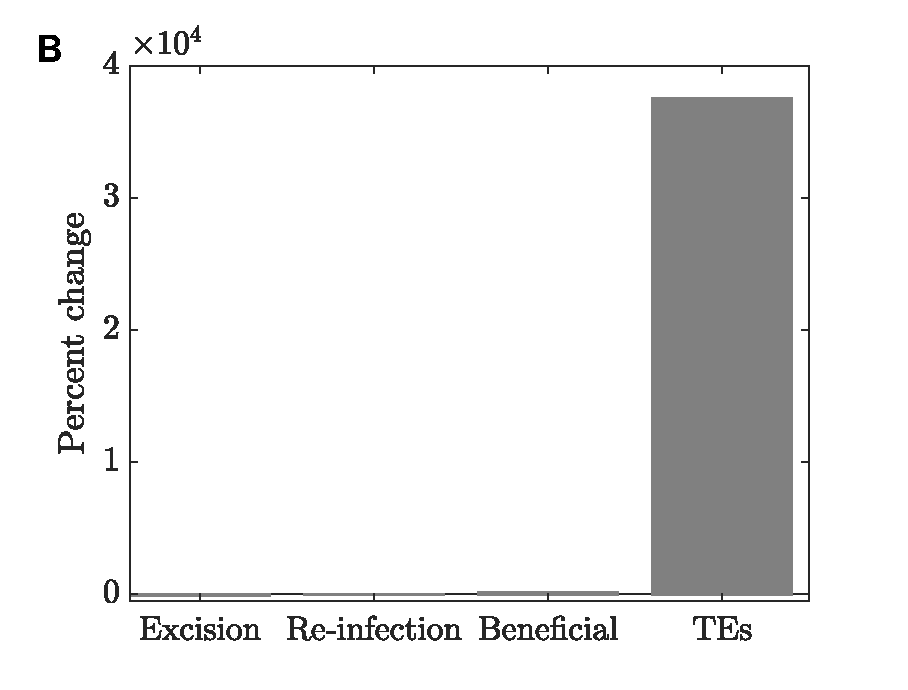
\includegraphics[scale=0.50]{BiTe2o.eps}
    \end{subfigure}\hfill\\  \begin{subfigure}[t]{0.50\textwidth}
        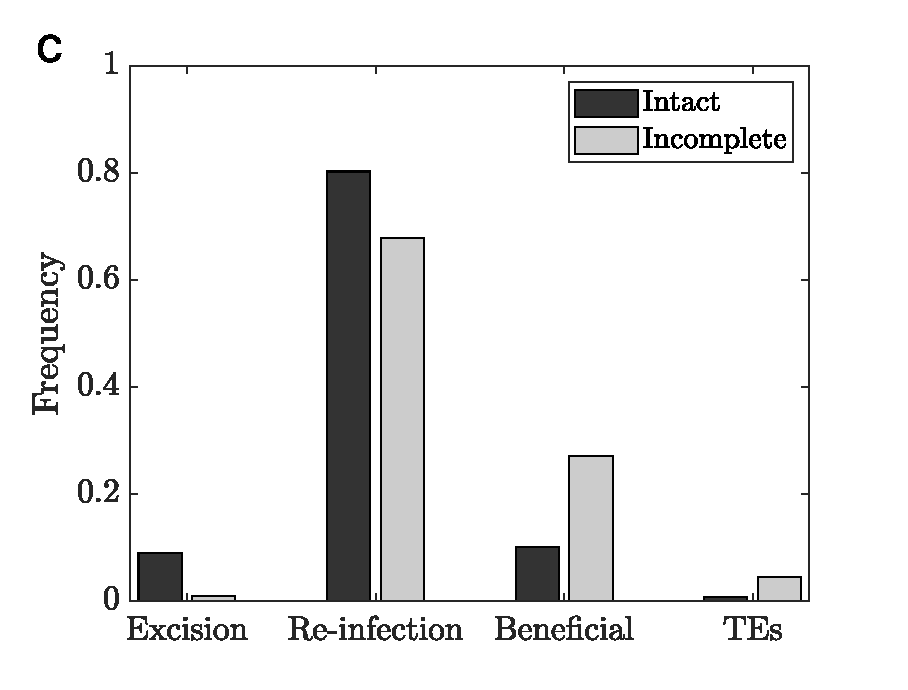
\includegraphics[scale=0.50]{BiTe190.eps}
    \end{subfigure}\hfill   \begin{subfigure}[t]{0.50\textwidth}
    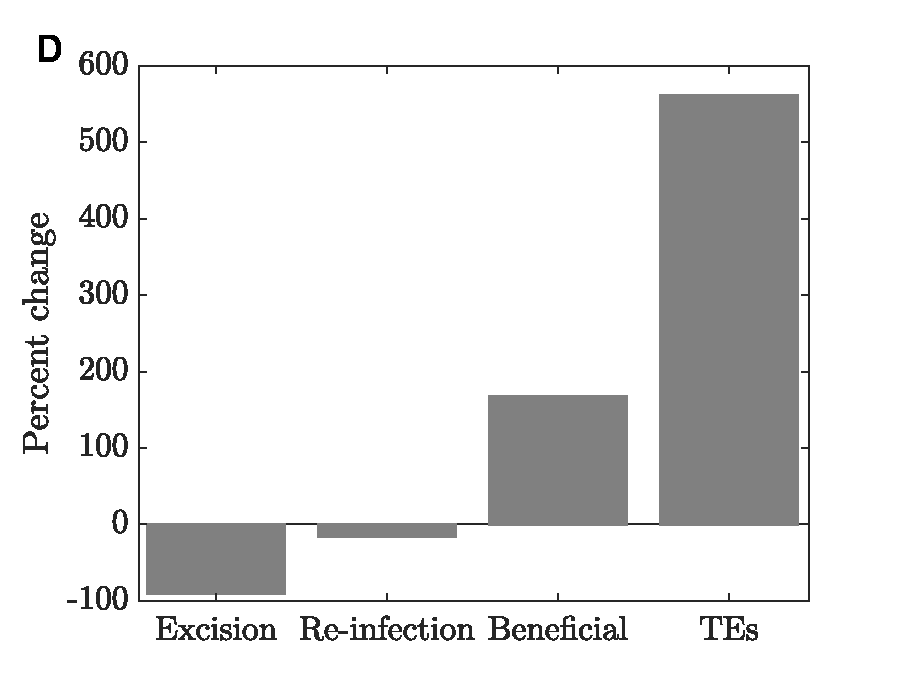
\includegraphics[scale=0.50]{BiTe290.eps}
    \end{subfigure} \hfill    
     \caption[Gene frequencies in intact and incomplete prophages, when TEs are included and intact prophagea are defined as sequences containing all the genes required for excision and reinfection.]{Gene frequencies in intact and incomplete prophages, when TEs are included ($r_S = 1.5, \, r_L = 1.5, \, r_D = 0.048, \, r_T = 0.002$). (A) Frequency of genes of each type in intact and incomplete prophages, for the computational model simulated at the persistence equilibrium with TE disruptions; (B) Percent change in gene frequency from intact to incomplete;  for (A) and (B) intact prophagea are defined as sequences containing all the genes required for excision and reinfection; (C) Frequency of genes of each type in intact and incomplete prophages, for the computational model simulated at the persistence equilibrium with TE; (D) Percent change in gene frequency from intact to incomplete; for (C) and (D) intact prophages are defined as sequences containing 90\% or more of the possible prophage genes.}
     \label{fig:Biresultso}
     \end{figure}
% %\addcontentsline{toc}{chapter}{Bibliography}
% \bibliographystyle{apa}
% \bibliography{refrence}